% !TEX root = ../../seminar.tex

\subsection{Answer Question}
\label{subsec:answer question}
One way to answer the research question is using existing evidence that needs to be critically appraised prior to drawing conclusions. This includes checking study design, study quality, relevance for the research question, as well as consistency between different studies. 

Rainer \etal found that students had problems critically appraising evidence. See table \ref{table:issuesEBSE} issues \ref{itm:issue2} and \ref{itm:issue6}. They suggest sensitizing students for biases to solve this issue \cite{Rainer2006}. There are several tools to support critical appraisal of studies. Figure \ref{fig:critical appraisal} shows a checklist containing important factors to consider when appraising a study.\\
Another tool is the \emph{GRADE approach} \cite{Atkins2004}, a grading system for studies that goes beyond simple hierarchies of study types. It was introduced for medicine and has been used in the software engineering domain \cite{Wohlin2013EvidenceProfile,Dyba2008}. GRADE is a well-defined method and differentiates between the quality of evidence and the strength of recommendation.

\begin{figure}
	\centering
	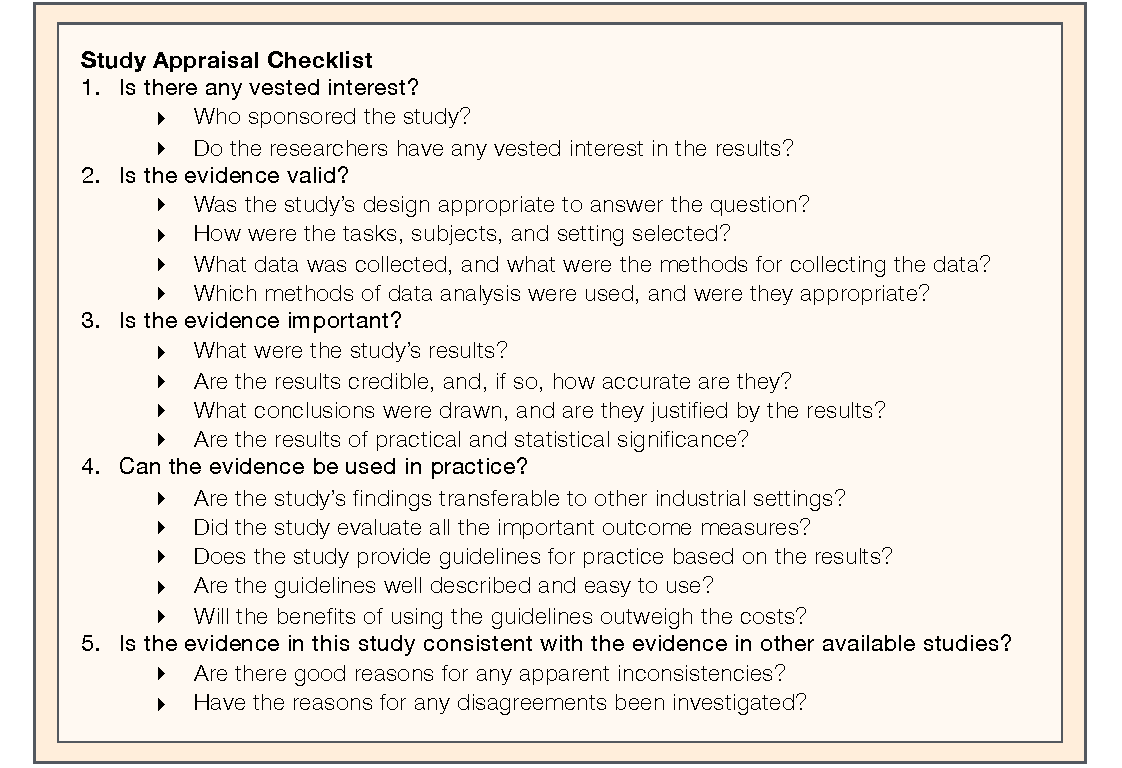
\includegraphics[width=12cm]{figures/study_appraisal.pdf}
\caption{Checklist for critical appraisal of studies compiled by Dyb{\aa} \etal \cite{Dyba2005}.}
\label{fig:critical appraisal}
\end{figure}

J{\o}rgensen \etal \cite{Jorgensen2016} reported indications of research and publication bias being quite common in the domain of software engineering. So, an important aspect of appraising studies is checking if they are biased. Shepperd presents similar findings and gives a good and short overview of the problem \cite{Shepperd2015}.

The critically appraised evidence (and the result of the conducted study) is used as foundation to accept or reject the hypothesis. Followed by answering the research question accordingly.





